\documentclass[12pt]{memoir}

\def\nsemestre {I}
\def\nterm {Spring}
\def\nyear {2024}
\def\nprofesor {Renzo Cavalieri}
\def\nsigla {DN}
\def\nsiglahead {Doctoral Notebook}
\def\nlang {ENG}
\def\ntrim{}

\input{../headerVarillyDiff}
%\newcommand{\Mickey}{\pre{\raisebox{-1mm}{\scalebox{1.3}{\ensuremath\bullet}}}\hspace{-1.8 mm}{\raisebox{-1.65mm}{\scalebox{2.1}{\ensuremath\bullet}}}^{\hspace{-2.1mm}\raisebox{-1mm}{\scalebox{1.3}{\ensuremath\bullet}}}}
\newcommand{\Mickey}{\pre{\raisebox{-1mm}{\scalebox{1.3}{\ensuremath\bullet}}}\hspace{-2.3 mm}{\raisebox{-1.65mm}{\scalebox{2.1}{\ensuremath\bullet}}}^{\hspace{-2.1mm}\raisebox{-1mm}{\scalebox{1.3}{\ensuremath\bullet}}}}
\newcommand{\Submickey}{\pre{\scalebox{0.75}{\ensuremath\bullet}}\hspace{-1.4mm}{\raisebox{-0.35mm}{\scalebox{1.1}{\ensuremath\bullet}}}^{\hspace{-1.1mm}\raisebox{-0.1mm}{\scalebox{0.75}{\ensuremath\bullet}}}}
\author{\nauthor}
\begin{document}

\section{My (?) theorem}

In the pseudostable case, we can calculate the same GW invariant, just that now the calculation is a bit different because of cusps.

\subsection{\(C^{\ps}(3,d)\)}

Let us compute the genus 3, degree \(d\) GW invariant:

\[\int_{[\ov{\cM}^\text{ps}_{3,0}(X,d\bt)]^\vir}1.\]

Ross \cite{DustyNotes} conjectures that the fundamental class localizes in a similar fashion as to the non-pseudostable case. We have

\[\int_{[\ov{\cM}^\text{ps}_{3,0}(X,d\bt)]^\vir}1=\int_{[\ov{\cM}^\text{ps}_{3,0}(\bP^1,d)]^\vir}e(H^1f^\ast\cO(-H))e(H^1f^\ast\cO(-H+t)).\]

The fixed maps consist of a \(\bP^1\) mapping as \(z\mapsto z^d\) together with positive genus components collapsing down to either \(0\) or \(\infty\). Such maps can be enumerated by ordered partitions of \(3\) with \(2\) parts, we have the fixed loci

\[F_{(3,0)},\quad F_{(2,1)},\quad F_{(1,2)},\word{and} F_{(0,3)}.\]

The fixed locus \(F_{(i,j)}\) denotes the nodal curve consisting of three components: one of genus \(i\) mapping to zero, the smooth component \(\bP^1\) and the genus \(j\) component mapping to infinity; this, along the information of the map. Let us analyze the contribution of \(F_{(3,0)}\).

\subsubsection{The \((3,0)\) contribution}

Instead of pulling back \(\cO(-H)\), we pullback \(\cO(-H+s+t)\) and then specialize to the cases \(s=0\) and \(s=-t\). Let \(C\) be the curve in question, its normalization sequence is

\[0\to\cO_C\to \cO_{g=3}\oplus\cO_{\bP^1}\to\un\bC_{\text{node}}\to 0\]

where \(\cO_{g=3}\) is the trivial sheaf over the genus 3 component. Tensoring with \(f^\ast\cO(-H+s+t)\) returns

\[0\to f^\ast\cO(-H+s+t)\to \cO(s)\oplus\cO(-d\widetilde{H}+s+t)\to\genr{(s)}\to 0.\]

Taking long exact sequence in cohomology via \(H^\ast(C,-)\) gives us

\[%%Fix overful
    \begin{tikzcd}[column sep=tiny, row sep=tiny]
        0 \arrow[r]\ar[draw=none]{d}[name=X, anchor=center]{} &
        H^0(f^\ast \cO(-H+s+t)) \arrow[r] &
        H^0(\cO(s))\oplus H^0(\cO(-d\widetilde{H}+s+t)) \arrow[r] &
        H^0(\genr{(s)})
        \ar[rounded corners, to path={ -- ([xshift=2ex]\tikztostart.east) |- (X.center) \tikztonodes -| ([xshift=-2ex]\tikztotarget.west) -- (\tikztotarget)}]{dll}[at end]{}\\[1ex]
        & H^1(f^\ast \cO(-H+s+t)) \arrow[r] &
        H^1(\cO(s))\oplus H^1(\cO(-d\widetilde{H}+s+t)) \arrow[r] &
        0
    \end{tikzcd}
\]

Observe that the two negative bundles have zero \(H^0\), then taking Euler classes and cancelling \(H^0(\cO(s))\) with \(H^0(\genr{(s)})\)'s we obtain
\begin{align*}
    e\bigl(H^1(f^\ast \cO(-H+s+t))\bigr) & =e\bigl(H^1(\cO(s))\bigr)e\bigl(H^1(\cO(-d\widetilde{H}+s+t))\bigr)                                         \\
                                         & =\bigl(s^3+(-\la_1^{\ps})s^2+\la_2^{\ps} s+(-\la_3^{\ps})\bigr)\left(\prod_{k=1}^{d-1}s+\frac{kt}{d}\right)
\end{align*}
where we used that

\[H^1(\cO(s))\isom \bE^\vee\ox H^0(\cO(s)),\]

via Serre duality. Specializing this quantity to \(s=-t\) and \(s=0\) and taking the product recovers the initial desired product pulledback to \(F_{(3,0)}\). We have
\begin{align*}
      & i_{(3,0)}^\ast(e(H^1f^\ast\cO(-H))e(H^1f^\ast\cO(-H+t)))                                                                                                                \\
    = & \bigl(-\la_3^{\ps}\bigr)\left(\prod_{k=1}^{d-1}\frac{kt}{d}\right)\bigl(-t^3-\la_1^{\ps}t^2-\la_2^{\ps}t-\la_3^{\ps}\bigr)\left(\prod_{k=1}^{d-1}-t+\frac{kt}{d}\right) \\
    = & \la_3^{\ps}\bigl(t^3+\la_1^{\ps}t^2+\la_2^{\ps}t+\la_3^{\ps}\bigr)(-1)^{d-1}\left(\frac{t}{d}\right)^{2d-2}(d-1)!^2.
\end{align*}

\hrule

\begin{Rmk}\label{rmk-new-notn-hom-lambda}
    We would like to use the notation \(\La_g^{\ps}(k)\) from \cite{MattAndRenzo} which is

    \[\La_g^{\ps}(k)=\sum_{i=0}^{g}k^i\la_i^{\ps}.\]

    Evaluating at \(k=1\) returns the total Chern class of the Hodge bundle and at \(-1\), the dual's. Observe that the second quantity in our result is not exactly the total Chern class, but the \emph{homogeneous} version.\par
    Perhaps we should introduce new notation to be

    \[\La_g^{\ps}(k,\l)=\sum_{i=0}^{g}k^i\la_i^{\ps}\l^{g-i}\]

    so that our quantity is \(\La_g^{\ps}(1,t)\). The quantity \(\La_g^{\ps}(k,\l)\) can even be expressed as a convolution of two sequences


    \[\La_g^{\ps}(k,\l)= \bigl((k^i\la_i^{\ps})_i\ast(\l^i)_i\bigr)(g)
    \]


    In particular, we may express the series whose general term is \(\La_g^{\ps}(k,\l)\) as the product of two series:

    \[\sum_{g=0}^{\infty}\La_g^{\ps}(k,\l)=\left(\sum_{g=0}^{\infty}k^g\la_g^{\ps}\right)\left(\sum_{g=0}^{\infty}\l^g\right)=\frac{\La_g^{\ps}(k)}{1-\l}.
    \]

    Indeed, the sum \(\La_g^{\ps}(k)\) is finite as there's no lambda class above the genus of the curve.
\end{Rmk}

\hrule

\begin{Rmk}[20251202, after meeting]
    Observe the lack of need to use the notation \(\La_g^{\ps}(k,\l)\). It suffices to redefine \(\La_g^{\ps}(k)\) as

    \[\La_g^{\ps}(k)\defeq\sum_{i=0}^{g}k^{g-i}\la_i^{\ps}.\]

    Then the old \(\La_g^{\ps}(1,t)\) is just the new \(\La_g^{\ps}(t)\). However the \(\La_g^{\ps}(-1,t)\) doesn't match up quite nicely with \(\La_g^{\ps}(-t)\). This last quantity is

    \[(-1)^gt^g+(-1)^{g-1}t^{g-1}\la_1^{\ps}+\dots+(-1)^0\la_g^{\ps}\]

    so that multiplying the whole quantity by \((-1)^g\), we change this expression to

    \[t^{g}-t^{g-1}\la_1+\dots+(-1)^g\la_g=\La_g^{\ps}(-1,t)\]

    as desired. We will thus stick with this notation

\end{Rmk}
\begin{ptcb}
    The simplification of the products is done in the following fashion.
    \begin{align*}
          & \prod_{k=1}^{d-1}\left(-t+\frac{kt}{d}\right)\left(\frac{kt}{d}\right) \\
        = & \left(\frac{t}{d}\right)^{2d-2}(d-1)!\prod_{k=1}^{d-1}-d+k.
    \end{align*}
    Substituting \(-\l\) as \(-d+k\) we note that the product becomes

    \[\prod_{k=1}^{d-1}-d+k=\prod_{\l=d+1}^{1}-\l=(-1)^{d-1}(d-1)!\]

    so that combining with the previous amount we get

    \[(-1)^{d-1}\left(\frac{t}{d}\right)^{2d-2}(d-1)!^2\]

\end{ptcb}

We are left with analyzing the normal bundle to \(F_{(3,0)}\) inside the moduli space. As in the stable case, going through the tangent-normal sequence and using deformation theory to relate cohomology with the particular bundles we get

\[e(N_{(3,0)})=\frac{e(\DefB(f))e(\DefB(C))}{e(\Aut(C))e(\Ob(f))}\]

and each equivariant Euler class only contributes its moving part.
\begin{itemize}
    \item The dual graph of the curve has one valence one vertex, it corresponds to the only smooth point of the curve. It lies over infinity so its contribution to the automorphisms bundle is

          \[e(\Aut(C))=-\frac{t}{d}.\]

    \item In this case, the deformations of the curve come from the curve's normalization. Let \(P,Q\) be the points in positive genus and smooth components respectively which map to the node. The Euler class then is

          \[e(\DefB(C))=-\psi_P-\psi_Q=-\psi_P+\frac{t}{d}\]

          as the negative psi class corresponds to \(c_1\) of the \emph{tangent} bundle. So it is the tangent weight at the point in question.
    \item The map's deformations and obstructions come from the same sequence. Tensoring the normalization sequence with \(f^\ast T\bP^1\) we get

          \[0\to f^\ast T\bP^1\to \cO(t)\oplus\cO(2d\widetilde{H}-t)\to\genr{(t)}\to 0.\]

          Now the long sequence in cohomology contains the desired bundles as

          \[%%Fix overful
              \begin{tikzcd}[column sep=tiny, row sep=tiny]
                  0 \arrow[r] &
                  \DefB(f) \arrow[r] &
                  H^0(\cO(t))\oplus H^0(\cO(2d\widetilde{H}-t)) \arrow[r] &
                  H^0(\genr{(t)})
                  \ar[rounded corners, to path={ -- ([xshift=2ex]\tikztostart.east) |- (X.center) \tikztonodes -| ([xshift=-2ex]\tikztotarget.west) -- (\tikztotarget)}]{dll}[at end]{}\\[1ex]
                  & \Ob(f) \arrow[r] &
                  H^1(\cO(t))\oplus H^1(\cO(2d\widetilde{H}-t)) \arrow[r] &
                  0
              \end{tikzcd}
          \]

          Taking Euler classes, cancelling out terms and realizing the \(H^1\) of a positive bundle is zero gives us

          \[\frac{e(\DefB(f))}{e(\Ob(f))}=\frac{e\bigl(H^0(\cO(2d\widetilde{H}-t))\bigr)}{e\bigl(H^1(\cO(t))\bigr)}.\]

          \(H^0(\cO(2d\widetilde{H}-t))\) has \(2d+1\) middle sections and the one right in the middle is fixed, so we get \(2d\) contributions as

          \[e\bigl(H^0(\cO(2d\widetilde{H}-t))\bigr)=\prod_{\substack{k=0\\ k\neq d}}^{2d}t-\frac{kt}{d}=\left(\frac{t}{d}\right)^{2d}d!^2(-1)^d.\]

          \begin{ptcb}
              The simplification for this product goes along similar lines:
              \begin{align*}
                    & \prod_{\substack{k=0                                                             \\ k\neq d}}^{2d}t-\frac{kt}{d}\\
                  = & \left(\frac{t}{d}\right)^{2d}\prod_{\substack{k=0                                \\ k\neq d}}d-k\\
                  = & \left(\frac{t}{d}\right)^{2d}\bigl(d\.(d-1)\cdots 1\.(-1)\.(-2)\cdots (-d)\bigr) \\
                  = & \left(\frac{t}{d}\right)^{2d}d!^2(-1)^d.
              \end{align*}
          \end{ptcb}
          Again via Serre duality,

          \[e\bigl(H^1(\cO(t))\bigr)=t^3+(-\la_1^{\ps})t^2+\la_2^{\ps}t+(-\la_3^{\ps})=(-1)^3\La_3^{\ps}(-t).\]

\end{itemize}
We wrap everything up into

\[e(N_{(3,0)})=\frac{\bigl[\left(t/d\right)^{2d}d!^2(-1)^d\bigr]\bigl[-\psi_P+t/d\bigr]}{\bigl[(-1)^3\La_3^{\ps}(-t)\bigr]\bigl[-t/d\bigr]}.\]

and putting it together with the pullback of the Euler classes up top, we get

\begin{align*}
      & \frac{\bigl[(-1)^3\La_3^{\ps}(-t)\bigr]\bigl[-t/d\bigr]\bigl[\la_3^{\ps}\La_3^{\ps}(t)(-1)^{d-1}\left(t/d\right)^{2d-2}(d-1)!^2\bigr]}{\bigl[\left(t/d\right)^{2d}d!^2(-1)^d\bigr]\bigl[-\psi_P+t/d\bigr]} \\
    = & \frac{\bigl[(-1)^3\La_3^{\ps}(-t)\bigr]\bigl[-t/d\bigr]\bigl[\la_3^{\ps}\La_3^{\ps}(t)\bigr]}{\bigl[-t^2\bigr]\bigl[(t/d)(1-d\psi_P/t)\bigr]}                                                              \\
    = & \frac{\la_3^{\ps}\La_3^{\ps}(t)(-1)^3\La_3^{\ps}(-t)}{t^2(1-d\psi_P/t)}.
\end{align*}

\iffalse
    \hrule

    \begin{Qn}\label{qn-gnr-function-total-lambda}
        ¿How far can we stretch the generating function argument? In essence, we affirmed in the previous remark \ref{rmk-new-notn-hom-lambda} that

        \[\sum_{g=0}^{\infty}\La_g^{\ps}(-1,t)=\sum_{g\geq 0}t^g+(-\la_1^{\ps})t^{g-1}+\dots+(-1)^g\la_g^{\ps}=\frac{\La_g^{\ps}(-1)}{1-t}.
        \]

        Multiplying both terms as

        \[\frac{\La_g^{\ps}(1)\La_g^{\ps}(-1)}{(1-t)^2}\]

        does not yield the desired result because the series that we get has, as a general term, the convolution of \((\La_g^{\ps}(-1,t))_{g\geq 0}\) with \((\La_g^{\ps}(1,t))_{g\geq 0}\).\par
        Further development must be pursued.
    \end{Qn}


    \begin{ptcb}
        On the left, using Matt and Renzo's formula from \cite{MattAndRenzo} and homogenizing gives us

        \[t^6+t^4\glu^1_\ast\bigl(\psi_\star-\psi_\8\bigr)+\frac{t^2}{2}\glu^2_\ast\bigl((\psi_{\star_1}-\psi_{\8_1})(\psi_{\star_2}-\psi_{\8_2})\bigr)+\frac{1}{6}\glu^3_\ast(\dots).\]

        The right hand side on the other hand is the product of \(\frac{1}{(1-t)^2}\) with

        \[1+\glu^1_\ast\bigl(\psi_\star-\psi_\8\bigr)+\frac{1}{2}\glu^2_\ast\bigl((\psi_{\star_1}-\psi_{\8_1})(\psi_{\star_2}-\psi_{\8_2})\bigr)+\frac{1}{6}\glu^3_\ast(\dots).\]

        The series for \(\frac{1}{(1-t)^2}\) is

        \[\sum_{g=1}^{\infty}gt^{g-1}=\sum_{g=0}^\infty(g+1)t^g\]

        \begin{ptcb}
            Indeed observe that

            \[g+1=\sum_{i=0}^{g}1\.1\]

            and also via differentiation
        \end{ptcb}
        Taking the product of the sums

        \[\left(\sum_{g=0}^{\infty}\frac{1}{g!}\glu^g_\ast(\dots)\right)\left(\sum_{g=0}^{\infty}(g+1)t^g\right)\]

        means that we must take the convolution which is

        \[\sum_{g=0}^{\infty}\sum_{k=0}^{g}\frac{1}{k!}\glu_\ast^k(\dots)(g-k+1)t^{g-k}.\]

        The first few terms of the inner sum are

        \[(g+1)t^g+gt^{g-1}\glu^1_\ast(\cdots)+\frac{g-1}{2}t^{g-2}\glu^2(\cdots)+\cdots\]

        This quantity \textbf{does not coincide} with the upper quantity.\par
    \end{ptcb}

    \hrule
\fi


\begin{Rmk}
    Let us observe that the degree of the class in question is

    \[3+3+3-2=7\]

    which coincides with \(\dim\ov{\cM}^{\ps}_{3,1}=3(3)-3+1=7\), the dimension of the fixed locus \(F_{(3,0)}\).
\end{Rmk}

In the previous observation we have used the fact that \(\ov{\cM}^{\ps}_{g,n}\) has the same dimension as its stable counterpart. This is mentioned in \cite{RenzoAndCo}, pp.5. We won't limit ourselves to only using this fact, we need two more results to further the calculation.

\begin{Th}[\cite{RenzoAndCo}, T.2.4]\label{th-renzoco-defn-pslambda}
    If \(\cT\:\ov{\cM}_{g,n}\to\ov{\cM}^{\ps}_{g,n}\) is the ``contracting-eliiptic-tails'' morphism, then

    \[\cT^\ast(\la_j)=\sum_{k=0}^{j}\frac{1}{k!}\glu_{\ast}^k\bigl(p_0^\ast(\la_{j-k})\bigr)\]

\end{Th}

\begin{Th}[\cite{MattAndRenzo}, T.3.1]\label{th-matt-mumford-formula}
    The following relationship holds:

    \[\La_g^{\ps}(1)(-1)^g\La_g^{\ps}(-1)=\sum_{k=0}^{g}\frac{1}{k!}\glu_{\ast}^k\left(\prod_{j=1}^{k}\psi_{\star j}-\psi_{\8 j}\right).\]

\end{Th}

In the previous result, homogenizing the total lambda classes, homogenizes the right hand side as well. This means that

\[\La_g^{\ps}(t)(-1)^g\La_g^{\ps}(-t)=\sum_{k=0}^{g}\frac{t^{2g-2k}}{k!}\glu_{\ast}^k\left(\prod_{j=1}^{k}\psi_{\star j}-\psi_{\8 j}\right).
\]


Now, we just expand the pseudostable Mumford relation to obtain
\begin{align*}
      & \la_3^{\ps}\La_3^{\ps}(t)(-1)^3\La_3^{\ps}(-t)                                                                                                                                 \\
    = & \la_3^{\ps}\.\bigl(t^6+t^4\glu_\ast^1(\psi_\star-\psi_\8)+\tfrac{t^2}{2}\glu_\ast^2((\psi_{\star1}-\psi_{\81})(\psi_{\star2}-\psi_{\82}))+\tfrac{1}{6}\glu_\ast^3(\dots)\bigr)
\end{align*}

After distributing, it's sufficient to just analyze terms of the form
\begin{align*}
      & \la_3^{\ps}\.\glu_\ast^i\left(\prod_{j=1}^i(\psi_{\star j}-\psi_{\8j})\right)                                                                                                        \\
    = & \bigl(\la_3+\glu^1_\ast(p_0^\ast(\la_2))+\tfrac{1}{2}\glu^2_\ast(p_0^\ast(\la_1))+\tfrac{1}{6}\glu^3_\ast(1)\bigr)\.\glu_\ast^i\left(\prod_{j=1}^i(\psi_{\star j}-\psi_{\8j})\right)
\end{align*}
where \(i\) ranges from \(0\) to \(g\). This means that the first term of the resulting sum is just \(\la_3^{\ps}\).\par
Let us work with

\[\la_3^{\ps}\.\glu_\ast^1(\psi_\star-\psi_\8).\]


\begin{ptcb}
    For the first term:
    \begin{align*}
        \la_3\.\glu_\ast^1(\psi_\star-\psi_\8) & =\glu_\ast^1\bigl(p_0^\ast(\la_2)p_1^\ast(\la_1)(\psi_\star-\psi_\8)\bigr) \\
                                               & =\glu_\ast^1\bigl(p_0^\ast(\la_2)p_1^\ast(\la_1)\psi_\star\bigr)
    \end{align*}
    where we lose the term with \(\psi_\8\) because on \(\ov\cM_{1,1}\) we have a \(\la_1\psi_\8\).\par
    Now the second:
    \begin{align*}
          & \glu_\ast^1(p_0^\ast(\la_2))\.\glu_\ast^1(\psi_\star-\psi_\8)                                                                        \\
        = & \glu_\ast^1(p_0^\ast(\la_2)(\psi_\8^2-\psi_\star^2))+\glu_\ast^2\bigl(p_0^\ast(\la_1)p_2^\ast(\la_1)(\psi_{\star2}-\psi_{\82})\bigr) \\
        = & -\glu_\ast^1\bigl(p_0^\ast(\la_2)\psi_\star^2\bigr)+\glu_\ast^2\bigl(p_0^\ast(\la_1)p_2^\ast(\la_1)\psi_{\star2}\bigr)
    \end{align*}
    where we once again lose the corresponding \(\psi_\8\)'s because of codimension reasons.
\end{ptcb}

\begin{Qn}
    In the second term of the expansion

    \[\glu_\ast^1(p_0^\ast(\la_2))\.\glu_\ast^1(\psi_\star-\psi_\8),\]

    in the transverse intersection, ¿why doesn't that \(\glu^2\) carry a \(2\) factor?\par
    With \textbf{Kelsey}, we developed the formula for the coefficient to be

    \[\binom{\text{Edges of result}}{\text{LCS}}\binom{\text{SCS}}{\text{uncolored}}\binom{\text{LCS}}{\text{SCS}-\text{already colored}}\]

    where LCS/SCS stands for largest/smallest color set. The issue is that in this case the factor accompanying the \(\glu^2\) would be a 2 which is not the real answer. Revisions must be made to the coefficient formula.
\end{Qn}

\begin{ptcb}
    The next term is
    \begin{align*}
          & \glu_\ast^2(p_0^\ast(\la_1))\.\glu_\ast^1(\psi_\star-\psi_\8)                                                      \\
        = & 2\glu^2_\ast(p_0^\ast(\la_1)(\psi_{\81}^2-\psi_{\star1}^2))+\glu^3_\ast(p_3^\ast(\la_1)(\psi_{\star3}-\psi_{\83})) \\
        = & -2\glu^2_\ast(p_0^\ast(\la_1)\psi_{\star1}^2)+\glu^3_\ast(p_3^\ast(\la_1)\psi_{\star3})
    \end{align*}
    where we'll need to add a factor of \(\half\) because the lambda term carried it from it's own expansion. Different from this one, the next term doesn't need it because

    \[\glu_\ast^3(1)\.\glu_\ast^1(\psi_\star-\psi_\8)=3\glu_\ast^3(\psi_{\81}^2-\psi_{\star1}^2)=0.\]

\end{ptcb}

Gathering everything gives the equality

\begin{align*}
    \la_3^{\ps}\.\glu_\ast^1(\psi_\star-\psi_\8)= & \glu_\ast^1\bigl(p_0^\ast(\la_2)p_1^\ast(\la_1)\psi_\star\bigr)                                                        \\
                                                  & -\glu_\ast^1\bigl(p_0^\ast(\la_2)\psi_\star^2\bigr)+\glu_\ast^2\bigl(p_0^\ast(\la_1)p_2^\ast(\la_1)\psi_{\star2}\bigr) \\
                                                  & -\glu^2_\ast(p_0^\ast(\la_1)\psi_{\star1}^2)+\half\glu^3_\ast(p_3^\ast(\la_1)\psi_{\star3})
\end{align*}

In a similar fashion we compute the product


\[\la_3^{\ps}\.\glu_\ast^2\bigl((\psi_{\star1}-\psi_{\81})(\psi_{\star2}-\psi_{\82})\bigr).\]


\begin{ptcb}
    As before, after expanding \(\la_3^{\ps}\) we see that
    \begin{align*}
          & \la_3\.\glu_\ast^2\bigl((\psi_{\star1}-\psi_{\81})(\psi_{\star2}-\psi_{\82})\bigr)                                       \\
        = & \glu_\ast^2\bigl(p_0^\ast(\la_1)p_1^\ast(\la_1)p_2^\ast(\la_1)(\psi_{\star1}-\psi_{\81})(\psi_{\star2}-\psi_{\82})\bigr) \\
        = & \glu_\ast^2\bigl(p_0^\ast(\la_1)p_1^\ast(\la_1)p_2^\ast(\la_1)\psi_{\star1}\psi_{\star2}\bigr)
    \end{align*}
    The next term is
    \begin{align*}
          & \glu_\ast^1(p_0^\ast(\la_2))\.\glu_\ast^2\bigl((\psi_{\star1}-\psi_{\81})(\psi_{\star2}-\psi_{\82})\bigr)      \\
        = & 2\glu_\ast^2\bigl(p_0^\ast(\la_1)p_2^\ast(\la_1)(\psi_{\81}^2-\psi_{\star1}^2)(\psi_{\star2}-\psi_{\82})\bigr) \\
          & +\glu_\ast^3\bigl(p_2^\ast(\la_1)p_3^\ast(\la_1)(\psi_{\star2}-\psi_{\82})(\psi_{\star3}-\psi_{\83})\bigr)
    \end{align*}
    Observe that this term is immediately zero. On the first summand, no \(\psi_\8\) can survive on the elliptic tails so the only possibility is to have the \(\psi_\star\)'s on the main component. This adds 3 degrees to the already loaded \(M_{1,3}\) with a \(\la_1\). In total, codimension 4 on dimension 3 space makes the element vanish.\par
    Similarly, no \(\psi_\8\) survives the next term and the \(M_{0,4}\) main component would have a \(\psi_{\star2}\psi_{\star3}\) accompanying it, thus annihilating it.\par
    Now multiplying the \(2\) \(\glu^2\)'s together:
    \begin{align*}
          & \glu_\ast^2(p_0^\ast(\la_1))\.\glu_\ast^2\bigl((\psi_{\star1}-\psi_{\81})(\psi_{\star2}-\psi_{\82})\bigr) \\
        = & 2\glu_\ast^2\bigl(p_0^\ast(\la_1)(\psi_{\81}^2-\psi_{\star1}^2)(\psi_{\82}^2-\psi_{\star2}^2)\bigr)       \\
          & +4\glu_\ast^3\bigl(p_3^\ast(\la_1)(\psi_{\82}^2-\psi_{\star2}^2)(\psi_{\star3}-\psi_{\83})\bigr)
    \end{align*}
    Any term with a \(\psi_\8^2\) immediately vanishes and also any \(\psi_\8\) accompanying a lambda class. This leaves us with

    \[2\glu_\ast^2\bigl(p_0^\ast(\la_1)\psi_{\star1}^2\psi_{\star2}^2\bigr)-4\glu_\ast^3\bigl(p_3^\ast(\la_1)\psi^2_{\star2}\psi_{\star3}\bigr)\]

    The first term carries codimension 5 on its \(M_{1,3}\) component while the second one has codimension 3 on its \(M_{0,4}\) component. This immediately annihilates those terms making the product zero at once.
\end{ptcb}

\begin{Rmk}
    Notice that the excess codimension on the ``\(0^{\text{th}}\) component'' comes from the lack of codimension on the elliptic tails. The first term has two elliptic tails with no decorations, adding two codimensions to the otherwise perfectly fine 3 dimensions, and the second term as well carries two more classes than needed.
\end{Rmk}

\begin{ptcb}
    We come to the final term which is \(\glu_\ast^3(1)\). The product results in

    \[6\glu_\ast^3\bigl((\psi_{\82}^2-\psi_{\star2}^2)(\psi_{\83}^2-\psi_{\star3}^2)\bigr).\]

    As before, the \(\psi_{\8}^2\) terms vanish. This leaves us with an \(M_{0,4}\) carrying 4 psi classes. The three excess codimensions correspond to the three elliptic tails without decorations.
\end{ptcb}

We have verified that

\begin{align*}
      & \la_3^{\ps}\.\glu_\ast^2\bigl((\psi_{\star1}-\psi_{\81})(\psi_{\star2}-\psi_{\82})\bigr)       \\
    = & \la_3\.\glu_\ast^2\bigl((\psi_{\star1}-\psi_{\81})(\psi_{\star2}-\psi_{\82})\bigr)             \\
    = & \glu_\ast^2\bigl(p_0^\ast(\la_1)p_1^\ast(\la_1)p_2^\ast(\la_1)\psi_{\star1}\psi_{\star2}\bigr)
\end{align*}

For the final calculation we're looking at


\[\la_3^{\ps}\.\glu_\ast^3\bigl((\psi_{\star1}-\psi_{\81})(\psi_{\star2}-\psi_{\82})(\psi_{\star3}-\psi_{\83})\bigr).\]


The term with psi classes can be simplified to a linear combination of \(\glu_\ast^3(\psi_{\star a}\psi_{\8b}\psi_{\8c})\) for \(1\leq a,b,c\leq 3\) distinct plus a \(-\glu_\ast^3(\psi_{\81}\psi_{\82}\psi_{\83})\).

\begin{ptcb}
    Against the ordinary lambda class, none of those terms survive as they all carry at least one \(\psi_\8\).\par
    Multiplying the \(\glu_\ast^1(p_0^\ast(\la_2))\) term still returns a \(\glu^3_\ast(1)\) graph with one edge bicolored. The lambda class distributes into two tails as \(\la_1\)'s. At least one of the \(\psi_\8\)'s is in the same component as a \(\la_1\) in any of the cases, so the product is zero.\par
    Similarly for \(\glu_\ast^2(p_0^\ast(\la_1))\), the only case where the product could be non-zero is when the \(\la_1\) gets distributed into the elliptic tail corresponding to the \(\psi_{\star a}\). However, the other two edges would be bicolored giving \(\psi_{\8}^2\) terms which annihilate the elliptic tails or adding more \(\psi_{\star}\)'s to the \(M_{0,4}\) component. Both of these cases are zero.\par
    Finally multiplying a \(\glu_\ast^3(1)\) repeats all edges. The terms get annihilated either by excess \(\psi_{\8}^2\)'s or \(\psi_{\star}\)'s on the main component.
\end{ptcb}

Collecting everything together we get

\begin{align*}
      & \la_3^{\ps}\.\bigl(t^6+t^4\glu_\ast^1(\psi_\star-\psi_\8)+\tfrac{t^2}{2}\glu_\ast^2((\psi_{\star1}-\psi_{\81})(\psi_{\star2}-\psi_{\82}))+\tfrac{1}{6}\glu_\ast^3(\dots)\bigr)                  \\
    = & t^6\la_3^{\ps}                                                                                                                                                                                  \\
      & +t^4\Bigl(\glu_\ast^1\bigl(p_0^\ast(\la_2)p_1^\ast(\la_1)\psi_\star\bigr)-\glu_\ast^1\bigl(p_0^\ast(\la_2)\psi_\star^2\bigr)+\glu_\ast^2\bigl(p_0^\ast(\la_1)p_2^\ast(\la_1)\psi_{\star2}\bigr) \\
      & \qquad-\glu^2_\ast(p_0^\ast(\la_1)\psi_{\star1}^2)+\half\glu^3_\ast(p_3^\ast(\la_1)\psi_{\star3})\Bigr)                                                                                         \\
      & +\frac{t^2}{2}\glu_\ast^2\bigl(p_0^\ast(\la_1)p_1^\ast(\la_1)p_2^\ast(\la_1)\psi_{\star1}\psi_{\star2}\bigr)+0
\end{align*}

We may divide by the \(t^2\) term and then use the power series

\[\frac{1}{1-(d\psi_P/t)}=\sum_{k\geq 0}(d\psi_P/t)^k.\]

The only power that will survive is that which cancels the corresponding \(t\) in the expansion. This is because of codimension reasons: there's either too little or too much. Our expression becomes

\begin{align*}
     & d^4\la_3^{\ps}\psi_{P}^4+d^2\glu_\ast^1\bigl(p_0^\ast(\la_2)p_1^\ast(\la_1)\psi_\star\bigr)\psi_P^2+d^2(0)   \\
     & +\frac{d^0}{2}\glu_\ast^2\bigl(p_0^\ast(\la_1)p_1^\ast(\la_1)p_2^\ast(\la_1)\psi_{\star1}\psi_{\star2}\bigr)
\end{align*}

where the remaining terms accompanied by the \(d^2\) degree get cancelled after multiplying the psi class.\par
We may now calculate the integral corresponding to \(F_{(3,0)}\)'s contribution as
\begin{align*}
    I_{(3,0)}= & d^4\int_{\ov{M}^{\ps}_{3,1}}\la_3^{\ps}\psi_{P}^4+d^2\left(\int_{\ov{M}_{2,2}}\la_2\psi_P^2\psi_\star\right)\left(\int_{\ov{M}_{1,1}}\la_1\right) \\
               & +\half\left(\int_{\ov{M}_{1,3}}\la_1\psi_{\star1}\psi_{\star2}\right)\left(\int_{\ov{M}_{1,1}}\la_1\right)^2
\end{align*}
Citing a couple more results is the way to calculate this integrals. the first result is about the behaviour of linear Hodge integrals.

\begin{Th}[\cite{RenzoAndCo}, P.3.2]\label{th-renzoco-only-one-pslambda}
    For any \(j\in[g]\) and \(F\in\bZ[\un x]\),

    \[\int_{\ov{M}_{g,n}^{\ps}}\la_j^{\ps}F(\un{\psi})=\int_{\ov{M}_{g,n}}\la_jF(\un{\psi}).\]

\end{Th}

This tells us that the result of the first integral is

\[d^4b_3,\word{where}b_g=\frac{2^{2g-1}-1}{2^{2g-1}}\frac{|B_{2g}|}{(2g)!}\]

and \(B_g\) is the \(g^{\text{th}}\) Bernoulli number.\par
For the integrals with one lambda class, we use the result previously known as the \(\la_g\)-conjecture.

\begin{Th}[\cite{GetzlerAndPandharipande}, T.3]\label{th-lambdagConj}
    For \(k_1,\dots,k_n\) summing to \(2g+n-3\),

    \[\int_{\ov{M}_{g,n}}\psi_1^{k_1}\cdots\psi_n^{k_n}\la_g=\binom{2g+n-3}{k_1,\dots,k_n}b_g.\]

\end{Th}

This allows us to conclude that
\begin{align*}
    I_{(3,0)} & =d^4b_3+d^2\binom{4+2-3}{2,1}b_2\.\frac{1}{24}+\frac{1}{2}\binom{2+3-3}{1,1}b_1\.\frac{1}{24^2} \\
              & =d^4b_3+\frac{3d^2b_2}{24}+\frac{2b_1}{2\.24^2}
\end{align*}

\subsubsection{The \((2,1)\) contribution}

The calculation proceeds in a similar fashion. The curve \(C_{(2,1)}\) has a normalization sequence given by


\[0\to\cO_C\to \cO_{g=2}\oplus\cO_{\bP^1}\to\un\bC_{\text{node}}\oplus\un\bC_{\text{cusp}}x\to 0.\]
\par
In this case, \(\un{\bC}x\) is the structure sheaf of \(\Spec(\genr{x}/(x^2))\) \red{MUST ADD GOOD EXPLANATION ON WHY THIS IS THIS SHEAF, ¿why is the normalization sequence of cusp that? ¿why does the cusp normalize into such sheaf?}. Skipping my lack of understanding of cusps, we may tensor by \({\raisebox{-0.08em}{\scalebox{1.5}{\ensuremath\star}}}\defeq f^\ast\cO(-H+s+t)\) to get

\[0\to {\raisebox{-0.08em}{\scalebox{1.5}{\ensuremath\star}}}\to \cO(s)\oplus\cO(-d\widetilde{H}+s+t)\to\genr{(s)}\oplus(\un{\bC}x\ox\cO(s+t))\to 0.
\]

After simplifying the long exact sequence in cohomology we get

\begin{align*}
    0 & \to H^0(\cO(s))\to H^0(\genr{(s)})\oplus H^0(\un{\bC}x\ox\cO(s+t))                                                  \\
      & \to {\raisebox{-0.08em}{\scalebox{1.5}{\ensuremath\star}}}\to H^1(\cO(s))\oplus H^1(\cO(-d\widetilde{H}+s+t)) \to 0
\end{align*}
Taking Euler class returns

\begin{align*}
    e({\raisebox{-0.08em}{\scalebox{1.5}{\ensuremath\star}}}) & =e(H^1(\cO(s)))e(H^1(\cO(-d\widetilde{H}+s+t)))e(H^0(\un{\bC}x\ox\cO(s+t)))                                               \\
                                                              & =(s^2+(-\la_1^{\ps})s+\la_2^{\ps})\left(\prod_{k=1}^{d-1}\left(s+\frac{kt}{d}\right)\right)\left(-\frac{-t}{d}+s+t\right) \\
\end{align*}

\begin{Rmk}
    The Euler class of the tensor product is the sum of both classes, no question there. However, the reason as to why the Euler class of \(\un{\bC}x\) is \red{not clear}. The section \(x\) carries the dual tangent weight at the corresponding point. Since the cusp is located at \(\infty\) and the tangent weight there is \(\frac{-t}{d}\), we have that the Euler class is \(-\frac{-t}{d}\).
\end{Rmk}

Specializing into \(s=-t\) and \(s=0\) gives us the numerator
\begin{align*}
      & i_{(2,1)}^\ast(e(H^1f^\ast\cO(-H))e(H^1f^\ast\cO(-H+t)))                                                                                                                                     \\
    = & \La_2^{\ps}(t)\left(\prod_{k=1}^{d-1}\left(-t+\frac{kt}{d}\right)\right)\left(\frac{t}{d}\right)\la_2^{\ps}\left(\prod_{k=1}^{d-1}\left(\frac{kt}{d}\right)\right)\left(\frac{t}{d}+t\right) \\
    = & \la_2^{\ps}\La_2^{\ps}(t)\bigl((-1)^{d-1}\left({t}/{d}\right)^{2d-2}(d-1)!^2\bigr)\bigl((t/d)(t/d+t)\bigr)
\end{align*}

For the normal bundle we follow a similar procedure.
\begin{itemize}
    \item There's no smooth points, so there's no automorphisms. In this case, \(e(\Aut(C))=0\), but since this is not part of the \emph{moving} part of the Euler class, we don't consider it into the calculation.
    \item We get a contribution from the node at 0, connecting the rational part with the positive genus part, and one from the cusp.

          \[e(\DefB(C))=\left(-\psi_P+\frac{t}{d}\right)\.24\left(\frac{-t}{d}\right)^2\]

    \item Tensoring the normalization sequence with \(f^\ast T\bP^1\) we get

          \[0\to f^\ast T\bP^1\to \cO(t)\oplus\cO(2d\widetilde{H}-t)\to\genr{(t)}\oplus\bigl(\un{\bC}x\ox\cO(-t)\bigr)\to 0.\]

          Now the long sequence in cohomology contains the desired bundles as

          \[%%Fix overful
              \begin{tikzcd}[column sep=tiny, row sep=tiny]
                  0 \arrow[r] &
                  \DefB(f) \arrow[r] &
                  H^0(\cO(t))\oplus H^0(\cO(2d\widetilde{H}-t)) \arrow[r] &
                  H^0(\genr{(t)})\oplus H^0\bigl(\un{\bC}x\ox\cO(-t)\bigr)
                  \ar[rounded corners, to path={ -- ([xshift=2ex]\tikztostart.east) |- (X.center) \tikztonodes -| ([xshift=-2ex]\tikztotarget.west) -- (\tikztotarget)}]{dll}[at end]{}\\[1ex]
                  & \Ob(f) \arrow[r] &
                  H^1(\cO(t))\oplus H^1(\cO(2d\widetilde{H}-t)) \arrow[r] &
                  0
              \end{tikzcd}
          \]

          Taking Euler classes:
          \begin{align*}
              \frac{e(\DefB(f))}{e(\Ob(f))} & =\frac{e\bigl(H^0(\cO(2d\widetilde{H}-t))\bigr)}{e\bigl(H^0\bigl(\un{\bC}x\ox\cO(-t)\bigr)\bigr)e\bigl(H^1(\cO(t))\bigr)} \\
                                            & =\frac{\left(t/d\right)^{2d}d!^2(-1)^d}{\bigl(-(-t/d)+(-t)\bigr)\bigl((-1)^2\La_2^{\ps}(-t)\bigr)}
          \end{align*}
\end{itemize}

Condensing this with the deformations of the curve we get

\[e(N_{(2,1)})=\frac{\bigl[\left(t/d\right)^{2d}d!^2(-1)^d\bigr]\bigl[(-\psi_P+t/d)\.24(-t/d)^2\bigr]}{\bigl(t/d-t\bigr)\bigl((-1)^2\La_2^{\ps}(-t)\bigr)}
\]

whose degree is

\[(2d+1+2)-(1+2)=2d\]

which should match with the codimension of \(\ov{M}_{2,1}\) inside the space of maps. The way to check this without computing the dimension of the space of maps is by considering the whole quotient:
\begin{align*}
      & \frac{\la_2^{\ps}\La_2^{\ps}(t)\bigl((-1)^{d-1}\left({t}/{d}\right)^{2d-2}(d-1)!^2\bigr)(t/d)(t/d+t)(t/d-t)\La_2^{\ps}(-t)}{\bigl[\left(t/d\right)^{2d}d!^2(-1)^d\bigr]\bigl[(-\psi_P+t/d)\.24(-t/d)^2\bigr]} \\
    = & \frac{\la_2^{\ps}\La_2^{\ps}(t)\La_2^{\ps}(-t)\bigl((1/d)(1/d+1)(1/d-1)t^3\bigr)}{(-t^2)\bigl(24(t/d)^3(1-d\psi_P/t)\bigr)}                                                                                   \\
    = & \frac{d^2-1}{24}\.\frac{\la_2^{\ps}\La_2^{\ps}(t)\La_2^{\ps}(-t)}{t^2\bigl(1-d\psi_P/t\bigr)}                                                                                                                 \\
\end{align*}
which has degree 4, same as the dimension of \(\ov{M}_{2,1}\), \(3\.2-3+1=4\).\par
Using Matt's theorem \ref{th-matt-mumford-formula} we simplify this class as
\begin{align*}
      & \frac{\la_2^{\ps}}{\bigl(1-d\psi_P/t\bigr)}\sum_{k=0}^{2}\frac{t^{4-2k-2}}{k!}\glu_{\ast}^k\left(\prod_{j=1}^{k}\psi_{\star j}-\psi_{\8 j}\right) \\
    = & \sum_{k=0}^{2}\frac{d^{2-2k}}{k!}\la_2^{\ps}\glu_{\ast}^k\left(\prod_{j=1}^{k}\psi_{\star j}-\psi_{\8 j}\right)\psi_P^{2-2k}                      \\
    = & d^2\la_2^{\ps}\psi_P^2+\la_2^{\ps}\glu_\ast^{1}(\psi_\star-\psi_\8)+0
\end{align*}

\begin{Rmk}
    The last term is zero before even expanding the psi class.
\end{Rmk}

\begin{Ej}
    Show that \(\la_g^{\ps}\glu_{\ast}^g\left(\prod_{j=1}^{k}\psi_{\star j}-\psi_{\8 j}\right)\) is zero in general. ¿Can this be done by induction on the number of elliptic tails of \(\la_g^{\ps}\)'s terms?
\end{Ej}

\begin{ptcb}
    Let us begin with the first term in the expansion of the product,
    \[
        \la_g\glu_{\ast}^g\left(\prod_{j=1}^{k}\psi_{\star j}-\psi_{\8 j}\right).
    \]
    \(\la_g\) distributes into all the elliptic tails of \(\glu_{\ast}^g\left(\prod_{j=1}^{k}\psi_{\star j}-\psi_{\8 j}\right)\) as \(\la_1\).\par
    In the monomial expansion of \(\glu_{\ast}^g(\dots)\), all terms with any \(\psi_{\8j}\) are cancelled by the \(\la_1\) as they add two codimensions to an \(M_{1,1}\). The class decorating the \(\glu_\ast^g(1)\) is then
    \[
        \left(\psi_{\star1}\dots\psi_{\star g}\right)\left(p_1^\ast\la_1\dots p_g^\ast\la_1\right).
    \]
    On the main component of \(\glu_\ast^g(1)\), we have an \(M_{0,g+1}\) with dimension \(g-2\) and the \(\psi\) classes add \(g\) codimensions. This means that this term must also be zero.
    \tcbline
    Now in general consider
    \[
        \glu_\ast^i(p_0^\ast\la_{g-i})\glu_{\ast}^g\left(\prod_{j=1}^{k}\psi_{\star j}-\psi_{\8 j}\right).
    \]
    The resulting graph has \(g\) elliptic tails of which \(i\) are bicolored and carry a \(\psi_{\8}^2-\psi_\star^2\) each. Expanding monomially we get that terms with any \(\psi_{\8j}^2\) is zero so that we get a
    \[
        \prod_{j\in I}(-\psi_{\star j}^2),
    \]
    where \(I\) is the set of indices of the bicolored tails. The main component has dimension \(g-2\) and the aforementioned class adds \(2i\) codimensions. So, if \(2i>g-2\) this term is immediately zero.\par
    Assume then \(g\geq 2i+2\). The remaining \(g-i\) tails are the ones where the \(\la_{g-i}\) distributed into \(\la_1\)'s. In such tails we cannot have a \(\psi_{\8}\) term, so we in fact get another set of \(\psi_{\star}\)'s in the main component. This time it's \(g-i\) of them.\par
    The final class decorating our graph is
    \[
        \prod_{j\in I}(-\psi_{\star j}^2)\prod_{j\in I^c}\psi_{\star j}p_j^{\ast}\la_1
    \]
    which adds \(2i+(g-i)=g+i\) codimensions to the main component. As \(i\geq 0\) we have \(g+i\geq g-2\) so that the whole term is zero.\par
    This allows us to conclude the desired result.
\end{ptcb}
We end this segment by calculating the product of the pseudostable lambda class with the 1 elliptic tail graph:

\begin{align*}
      & \bigl(\la_2+\glu^1_\ast(p_0^\ast(\la_1))+\tfrac{1}{2}\glu^2_\ast(1)\bigr)\glu_\ast^{1}(\psi_\star-\psi_\8)                                 \\
    = & \glu_\ast^{1}(p_0^\ast(\la_1)p_1^\ast(\la_1)\psi_\star)                                                                                    \\
      & +\glu_\ast^{1}\bigl(p_0^\ast(\la_1)(\psi_{\8}^2-\psi_{\star}^2)\bigr)+\glu_\ast^{2}\bigl(p_2^{\ast}(\la_1)(\psi_{\star2}-\psi_{\82})\bigr) \\
      & +\half\bigl(2\glu_\ast^2\bigl(\psi_{\81}^2-\psi_{\star1}^2\bigr)\bigr)                                                                     \\
    = & \glu_\ast^{1}(p_0^\ast(\la_1)p_1^\ast(\la_1)\psi_\star)
\end{align*}

Here, most terms vanish for codimension reasons. Putting this together and integrating we get

\begin{align*}
      & d^2\int_{\ov{M}^{\ps}_{2,1}}\la_2^{\ps}\psi_{P}^2+\left(\int_{\ov{M}_{1,2}}\la_1\psi_\star\right)\left(\int_{\ov{M}_{1,1}}\la_1\right) \\
    = & d^2b_2+1/24^2
\end{align*}

where we used theorem \ref{th-renzoco-only-one-pslambda} once again for the first integral.\par
Mutiplying by the coefficient we left behind we get a final result for the contribution of \(F_{(2,1)}\)

\[I_{(2,1)}=\frac{d^2-1}{24}\left(d^2b_2+\frac{1}{24^2}\right).\]


\subsubsection{The \((1,2)\) contribution}

Analogous to the previous case, the normalization sequence is


\[0\to\cO_C\to \cO_{\bP^1}\oplus\cO_{g=2}\to\un\bC_{\text{cusp}}y\oplus\un\bC_{\text{node}}\to 0.\]


Tensoring by \({\raisebox{-0.08em}{\scalebox{1.5}{\ensuremath\star}}}\defeq f^\ast\cO(-H+s+t)\) returns


\[
    0\to {\raisebox{-0.08em}{\scalebox{1.5}{\ensuremath\star}}}\to \cO(-d\widetilde{H}+s+t)\oplus\cO(s+t)\to(\un{\bC}y\ox\cO(s))\oplus\genr{(s+t)}\to 0.
\]


As before, we simplify with some minor changes

\begin{align*}
    0 & \to H^0(\cO(s+t))\to  H^0(\un{\bC}y\ox\cO(s))\oplus H^0(\genr{(s+t)})                                                 \\
      & \to {\raisebox{-0.08em}{\scalebox{1.5}{\ensuremath\star}}}\to H^1(\cO(-d\widetilde{H}+s+t))\oplus H^1(\cO(s+t)) \to 0
\end{align*}

Taking Euler classes we get

\begin{align*}
    e({\raisebox{-0.08em}{\scalebox{1.5}{\ensuremath\star}}}) & =e(H^1(\cO(-d\widetilde{H}+s+t)))e(H^1(\cO(s+t)))e(H^0(\un{\bC}y\ox\cO(s)))                                                    \\
                                                              & =\left(\prod_{k=1}^{d-1}\left(s+\frac{kt}{d}\right)\right)((s+t)^2+(-\la_1^{\ps})(s+t)+\la_2^{\ps})\left(-\frac{t}{d}+s\right) \\
\end{align*}

Plugging in \(s=-t\) and \(s=0\) gives

\begin{align*}
      & i_{(1,2)}^\ast(e(H^1f^\ast\cO(-H))e(H^1f^\ast\cO(-H+t)))                                                                                                                                \\
    = & \prod_{k=1}^{d-1}\left(-t+\frac{kt}{d}\right)\la_2^{\ps}\left(-\frac{t}{d}-t\right)\prod_{k=1}^{d-1}\left(\frac{kt}{d}\right)\bigl((-1)^2\La_2^{\ps}(-t)\bigr)\left(-\frac{t}{d}\right) \\
    = & \la_2^{\ps}\La_2^{\ps}(-t)\bigl((-1)^{d-1}\left({t}/{d}\right)^{2d-2}(d-1)!^2\bigr)\bigl((t/d)(t/d+t)\bigr)
\end{align*}

On the side of the normal bundle we don't have automorphisms as there's not smooth points. For curve deformations we get


\[e(\DefB(C))=24\left(\frac{t}{d}\right)^2\left(-\psi_P+\frac{-t}{d}\right)\]


whereas for map deformations and obstructions we repeat the previous process of tensoring the normalization sequence and then taking cohomology. First we get


\[0\to f^\ast T\bP^1\to \cO(2d\widetilde{H}-t)\oplus\cO(-t)\to\bigl(\un{\bC}y\ox\cO(t)\bigr)\oplus\genr{(-t)}\to 0.\]


This gets us


\[%%Fix overful
    \begin{tikzcd}[column sep=tiny, row sep=tiny]
        0 \arrow[r] &
        \DefB(f) \arrow[r] &
        H^0(\cO(2d\widetilde{H}-t))\oplus H^0(\cO(-t)) \arrow[r] &
        H^0\bigl(\un{\bC}y\ox\cO(t)\bigr)\oplus H^0(\genr{(-t)})
        \ar[rounded corners, to path={ -- ([xshift=2ex]\tikztostart.east) |- (X.center) \tikztonodes -| ([xshift=-2ex]\tikztotarget.west) -- (\tikztotarget)}]{dll}[at end]{}\\[1ex]
        & \Ob(f) \arrow[r] &
        H^1(\cO(2d\widetilde{H}-t))\oplus H^1(\cO(-t))\arrow[r] &
        0
    \end{tikzcd}
\]


Taking Euler classes:

\begin{align*}
    \frac{e(\DefB(f))}{e(\Ob(f))} & =\frac{e\bigl(H^0(\cO(2d\widetilde{H}-t))\bigr)}{e\bigl(H^0\bigl(\un{\bC}y\ox\cO(t)\bigr)\bigr)e\bigl(H^1(\cO(-t))\bigr)} \\
                                  & =\frac{\left(t/d\right)^{2d}d!^2(-1)^d}{\bigl(-(t/d)+t\bigr)\La_2^{\ps}(t)}
\end{align*}

Our integrand then is

\begin{align*}
      & \frac{\la_2^{\ps}\La_2^{\ps}(-t)\bigl((-1)^{d-1}\left({t}/{d}\right)^{2d-2}(d-1)!^2\bigr)(t/d)(t/d+t)(-t/d+t)\La_2^{\ps}(t)}{\bigl[\left(t/d\right)^{2d}d!^2(-1)^d\bigr]24(t/d)^2(-\psi_P-t/d)} \\
    = & \frac{\la_2^{\ps}\La_2^{\ps}(-t)\La_2^{\ps}(t)\bigl((t/d)^3(d^2-1)\bigr)}{(-t^2)24(t/d)^2(-t/d)\bigl(1-(-d\psi_P/t)\bigr)}                                                                      \\
    = & \frac{d^2-1}{24}\.\frac{\la_2^{\ps}\La_2^{\ps}(-t)\La_2^{\ps}(t)}{t^2\bigl(1-(-d\psi_P/t)\bigr)}
\end{align*}

Simplifying again via theorem \ref{th-matt-mumford-formula} we notice that the negative coefficient on the psi class cancels due to the even powers it is raised to

\begin{align*}
      & \frac{\la_2^{\ps}}{\bigl(1-(-d\psi_P/t)\bigr)}\sum_{k=0}^{2}\frac{t^{4-2k-2}}{k!}\glu_{\ast}^k\left(\prod_{j=1}^{k}\psi_{\star j}-\psi_{\8 j}\right) \\
    = & \sum_{k=0}^{2}\frac{(-d)^{2-2k}}{k!}\la_2^{\ps}\glu_{\ast}^k\left(\prod_{j=1}^{k}\psi_{\star j}-\psi_{\8 j}\right)(-\psi_P)^{2-2k}                   \\
    = & d^2\la_2^{\ps}\psi_P^2+\la_2^{\ps}\glu_\ast^{1}(\psi_\star-\psi_\8)
\end{align*}

Thus


\[I_{(1,2)}=I_{(2,1)}=\frac{d^2-1}{24}\left(d^2b_2+\frac{1}{24^2}\right)\]


\subsubsection{The \((0,3)\) contribution}

We may expedite the calculation following the first case. First the normalization sequence


\[0\to\cO_C\to \cO_{\bP^1}\oplus\cO_{g=3}\to\un\bC_{\text{node}}\to 0\]


then tensoring with \(f^\ast\cO(-H+s+t)\)


\[0\to f^\ast\cO(-H+s+t)\to \cO(-d\widetilde{H}+s+t)\oplus\cO(s+t)\to\genr{(s+t)}\to 0.\]


Further, the long exact sequence in cohomology is

\begin{align*}
    0                                                          & \to H^0(\cO(s+t))\to H^0(\genr{(s+t)})                      \\
    \to {\raisebox{-0.08em}{\scalebox{1.5}{\ensuremath\star}}} & \to H^1(\cO(s+t))\oplus H^1(\cO(-d\widetilde{H}+s+t)) \to 0
\end{align*}

so that the desired Euler class is the product

\begin{align*}
      & e(H^1(\cO(s+t)))e(H^1(\cO(-d\widetilde{H}+s+t)))                                                                                \\
    = & \bigl((s+t)^3+(s+t)^2(-\la_1^{\ps})+(s+t)\la_2^{\ps}-\la_3^{\ps}\bigr)\left(\prod_{k=1}^{d-1}\left(s+\frac{kt}{d}\right)\right)
\end{align*}

Plugging \(s=-t\), \(s=0\) returns

\begin{align*}
      & i_{(3,0)}^\ast(e(H^1f^\ast\cO(-H))e(H^1f^\ast\cO(-H+t)))                                                                                                                  \\
    = & \bigl(-\la_3^{\ps}\bigr)\left(\prod_{k=1}^{d-1}\frac{kt}{d}\right)\bigl(t^3+t^2(-\la_1^{\ps})+t\la_2^{\ps}-\la_3^{\ps}\bigr)\left(\prod_{k=1}^{d-1}-t+\frac{kt}{d}\right) \\
    = & (-\la_3^{\ps})(-1)^3\La_3^{\ps}(-t)(-1)^{d-1}\left(\frac{t}{d}\right)^{2d-2}(d-1)!^2.
\end{align*}

For the normal bundle:

\begin{itemize}
    \item The smooth point above zero gives us

          \[e(\Aut(C))=t/d.\]

    \item The deformations of the curve give

          \[e(\DefB(C))=-\psi_P+\frac{-t}{d}.\]

    \item For deformations and obstructions of the map we tensor the normalization sequence

          \[0\to f^\ast T\bP^1\to \cO(2d\widetilde{H}-t)\oplus\cO(-t)\to\genr{(-t)}\to 0.\]

          Taking cohomology gets us

          \[\begin{tikzcd}[column sep=tiny, row sep=tiny]
                  0 \arrow[r] &
                  \DefB(f) \arrow[r] &
                  H^0(\cO(2d\widetilde{H}-t))\oplus H^0(\cO(-t)) \arrow[r] &
                  H^0(\genr{(-t)})
                  \ar[rounded corners, to path={ -- ([xshift=2ex]\tikztostart.east) |- (X.center) \tikztonodes -| ([xshift=-2ex]\tikztotarget.west) -- (\tikztotarget)}]{dll}[at end]{}\\[1ex]
                  & \Ob(f) \arrow[r] &
                  H^1(\cO(-t)) \arrow[r] &
                  0
              \end{tikzcd}
          \]

          which gives

          \[\frac{e(\DefB(f))}{e(\Ob(f))}=\frac{e(H^0(\cO(2d\widetilde{H}-t)))}{e(H^1(\cO(-t)))}=\frac{\left(t/d\right)^{2d}d!^2(-1)^d}{(-1)^3\La_3^{\ps}(t)}\]

\end{itemize}

so that putting all together gets


\[e(N_{(0,3)})=\frac{\bigl[\left(t/d\right)^{2d}d!^2(-1)^d\bigr]\bigl[-\psi_P-t/d\bigr]}{\bigl[(-1)^3\La_3^{\ps}(t)\bigr]\bigl[t/d\bigr]}.\]


The integrand is then

\begin{align*}
      & \frac{\bigl[(-\la_3^{\ps})(-1)^3\La_3^{\ps}(-t)(-1)^{d-1}\left(t/d\right)^{2d-2}(d-1)!^2\bigr]\bigl[(-1)^3\La_3^{\ps}(t)\bigr]\bigl[t/d\bigr]}{\bigl[\left(t/d\right)^{2d}d!^2(-1)^d\bigr]\bigl[-\psi_P-t/d\bigr]} \\
    = & \frac{\bigl(\la_3^{\ps}\La_3^{\ps}(t)(-1)^3\La_3^{\ps}(-t)\bigr)(t/d)}{(-t^2)(-t/d)\bigl(1-(-d\psi_P/t)\bigr)}                                                                                                     \\
    = & \frac{\la_3^{\ps}\La_3^{\ps}(t)(-1)^3\La_3^{\ps}(-t)}{t^2\bigl(1-(-d\psi_P/t)\bigr)}.
\end{align*}

\iffalse
    We may expand using Matt's theorem \ref{th-matt-mumford-formula} to obtain

    \begin{align*}
          & \frac{\la_3^{\ps}}{1-(-d\psi_P/t)}\sum_{k=0}^{3}\frac{t^{6-2k-2}}{k!}\glu_{\ast}^k\left(\prod_{j=1}^{k}\psi_{\star j}-\psi_{\8 j}\right) \\
        = & \sum_{k=0}^{3}\frac{d^{6-2k-2}}{k!}\la_3^{\ps}\glu_{\ast}^k\left(\prod_{j=1}^{k}\psi_{\star j}-\psi_{\8 j}\right)\psi_P^{6-2k-2}         \\
        = & d^4\la_3^{\ps}\psi_P^4+d^2\glu_\ast^1\bigl(p_0^\ast(\la_2)p_1^\ast(\la_1)\psi_\star\bigr)\psi_P^2                                        \\
          & +\half\glu_\ast^2\bigl(p_0^\ast(\la_1)p_1^\ast(\la_1)p_2^\ast(\la_1)\psi_{\star1}\psi_{\star2}\bigr)
    \end{align*}
\fi

Because the psi class only obtains even powers, this calculation is exactly the same as in the \((3,0)\) case. We conclude that


\[I_{(0,3)}=I_{(3,0)}=d^4b_3+\frac{3d^2b_2}{24}+\frac{2b_1}{2\.24^2}.\]


The final result is

\begin{align*}
    C^{\ps}(3,d)= & \frac2d\left(d^4b_3+\frac{3d^2b_2}{24}+\frac{2b_1}{2\.24^2}\right)+\frac2d\left(\frac{d^2-1}{24}\left(d^2b_2+\frac{1}{24^2}\right)\right) \\
    =             & \frac{d^3}{6048}+\frac{d}{2880}=C(3,d)\left(1+\frac{21}{10d^2}\right)
\end{align*}

\subsection{The general case, \(C^{\ps}(g,d)\)}

Contributing maps here are enumerated by pairs \((g_1,g_2)\) with \(g_1+g_2=g\) and \(g_1,g_2\geq0\). These are ordered partitions of \(g\). We study the general case \(g_1,g_2\) with \(g_1\neq g-1,0\) and we treat these ones separately.

\subsubsection{The \((g_1,g_2)\) contribution}

The curve \(C_{(g_1,g_2)}\) has the normalization sequence
\[0\to\cO_C\to\cO_{g_1}\oplus\cO_{\bP^1}\oplus\cO_{g_2}\to\un{\bC}_{n_1}\oplus\un{\bC}_{n_2}\to0.\]
Tensoring with \(\Mickey\defeq f^\ast\cO(-H+s+t)\) gives

\[0\to \Mickey\to \cO(s)\oplus\cO(-d\widetilde{H}+s+t)\oplus\cO(s+t)\to\genr{(s)}\oplus\genr{(s+t)}\to 0.\]

After taking the long exact sequence in cohomology and simplifying, we're left with
\begin{align*}
    0                & \to H^0(\cO(s))\oplus H^0(\cO(s+t))\to H^0(\genr{(s)})\oplus H^0(\genr{(s+t)}) \\
    \to H^1(\Mickey) & \to H^1(\cO(s))\oplus H^1(\cO(-d\widetilde{H}+s+t))\oplus H^1(\cO(s+t))\to 0
\end{align*}
Taking Euler classes gives us
\begin{align*}
    e(H^1(\Mickey)) & =e\bigl(H^1(\cO(s))\bigr)e\bigl(H^1(\cO(-d\widetilde{H}+s+t))\bigr)e\bigl(H^1(\cO(s+t))\bigr)                            \\
                    & =(-1)^{g_1}\La_{g_1}^{\ps}(-s)\left(\prod_{k=1}^{d-1}\left(s+\frac{kt}{d}\right)\right)(-1)^{g_2}\La_{g_2}^{\ps}(-(s+t))
\end{align*}

We find the numerator by plugging in \(s=-t\), \(s=0\) and multiplying.

\begin{align*}
      & i_{(g_1,g_2)}^\ast(e(H^1f^\ast\cO(-H))e(H^1f^\ast\cO(-H+t)))                                                                                                                                       \\
    = & (-1)^{g_1}\La_{g_1}^{\ps}(t)\prod_{k=1}^{d-1}\left(-t+\frac{kt}{d}\right)(-1)^{g_2}\la_{g_2}^{\ps}(-1)^{g_1}\la_{g_1}^{\ps}\prod_{k=1}^{d-1}\left(\frac{kt}{d}\right)(-1)^{g_2}\La_{g_2}^{\ps}(-t) \\
    = & \bigl((-1)^{d-1}\left({t}/{d}\right)^{2d-2}(d-1)!^2\bigr)\bigl(\la_{g_1}^{\ps}\La_{g_1}^{\ps}(t)\bigr)\bigl(\la_{g_2}^{\ps}\La_{g_2}^{\ps}(-t)\bigr)
\end{align*}

There's no automorphisms as there's no smooth points so that the normal bundle only considers deformations and obstructions. In this case

\[e(\DefB(C))=(-\psi_{P_1}-\psi_{Q_1})(-\psi_{P_2}-\psi_{Q_2})=\left(-\psi_{P_1}+\frac{t}{d}\right)\left(-\psi_{P_2}+\frac{-t}{d}\right)\]

For the map, we tensor the normalization sequence by \(f^\ast T\bP^1\) to get

\[0\to f^\ast T\bP^1\to \cO(t)\oplus\cO(2d\widetilde{H}-t)\oplus\cO(-t)\to\genr{(t)}\oplus\genr{(-t)}\to 0.\]

Taking cohomology gets us

\[\begin{tikzcd}[column sep=tiny, row sep=tiny]
        0 \arrow[r] &
        \DefB(f) \arrow[r] &H^0(\cO(t))\oplus
        H^0(\cO(2d\widetilde{H}-t))\oplus H^0(\cO(-t)) \arrow[r] &
        H^0(\genr{(t)})\oplus H^0(\genr{(-t)})
        \ar[rounded corners, to path={ -- ([xshift=2ex]\tikztostart.east) |- (X.center) \tikztonodes -| ([xshift=-2ex]\tikztotarget.west) -- (\tikztotarget)}]{dll}[at end]{}\\[1ex]
        & \Ob(f) \arrow[r] &
        H^1(\cO(t))\oplus H^1(\cO(-t)) \arrow[r] &
        0
    \end{tikzcd}\]

thus the desired quotient of Euler classes is

\[\frac{e(\DefB(f))}{e(\Ob(f))}=\frac{e(H^0(\cO(2d\widetilde{H}-t)))}{e(H^1(\cO(t)))e(H^1(\cO(-t)))}=\frac{\left(t/d\right)^{2d}d!^2(-1)^d}{(-1)^{g_1}\La_{g_1}^{\ps}(-t)(-1)^{g_2}\La_{g_2}^{\ps}(t)}.\]

We end by condensing everything into the integrand.

\begin{align*}
      & \frac{\bigl((-1)^{d-1}\left({t}/{d}\right)^{2d-2}(d-1)!^2\bigr)\bigl(\la_{g_1}^{\ps}\La_{g_1}^{\ps}(t)\bigr)\bigl(\la_{g_2}^{\ps}\La_{g_2}^{\ps}(-t)\bigr)(-1)^{g_1}\La_{g_1}^{\ps}(-t)(-1)^{g_2}\La_{g_2}^{\ps}(t)}{\left(t/d\right)^{2d}d!^2(-1)^d\left(-\psi_{P_1}+t/d\right)\left(-\psi_{P_2}+({-t}/{d})\right)} \\
    = & \frac{\bigl(\la_{g_1}^{\ps}\La_{g_1}^{\ps}(t)(-1)^{g_1}\La_{g_1}^{\ps}(-t)\bigr)\bigl(\la_{g_2}^{\ps}\La_{g_2}^{\ps}(-t)(-1)^{g_2}\La_{g_2}^{\ps}(t)\bigr)}{(-t^2)\left(-\psi_{P_1}+t/d\right)\left(-\psi_{P_2}+({-t}/{d})\right)}                                                                                   \\
    = & {d^2}\left(\frac{\la_{g_1}^{\ps}\La_{g_1}^{\ps}(t)(-1)^{g_1}\La_{g_1}^{\ps}(-t)}{t^2\left(1-d\psi_{P_1}/t\right)}\right)\left(\frac{\la_{g_2}^{\ps}\La_{g_2}^{\ps}(-t)(-1)^{g_2}\La_{g_2}^{\ps}(t)}{t^2\left(1-(-d\psi_{P_2}/t)\right)}\right).
\end{align*}

We've seen before the minus sign on the psi class has no effect because of even powers. In this case, we just treat a general term of genus \(g\). Expanding via Matt's relation (theorem \ref{th-matt-mumford-formula}) gets us to

\begin{align*}
      & \frac{\la_{g}^{\ps}\La_{g}^{\ps}(t)(-1)^{g}\La_{g}^{\ps}(-t)}{t^2\left(1-d\psi_{P}/t\right)}                                                             \\
    = & \frac{\la_{g}^{\ps}}{t^2\left(1-d\psi_{P}/t\right)}\sum_{k=0}^{g}\frac{t^{2g-2k}}{k!}\glu_{\ast}^k\left(\prod_{j=1}^{k}\psi_{\star j}-\psi_{\8 j}\right) \\
    = & \sum_{k=0}^{g}\frac{d^{2g-2k-2}}{k!}\la_g^{\ps}\glu_{\ast}^k\left(\prod_{j=1}^{k}\psi_{\star j}-\psi_{\8 j}\right)\psi_{P}^{2g-2k-2}                     \\
    = & \sum_{k=0}^{g}\frac{d^{2g-2k-2}}{k!}\glu_\ast^k\left(p_0^\ast(\la_{g-k})\prod_{j=1}^{k}\psi_{\star j}p_j^\ast(\la_1)\right)\psi_{P}^{2g-2k-2}
\end{align*}
\hrule
\begin{Ej}
    The product
    \[
        \la_g^{\ps}\glu_{\ast}^k\left(\prod_{j=1}^{k}\psi_{\star j}-\psi_{\8 j}\right)\psi_{P}^{2g-2k-2}
    \]
    results in
    \begin{align*}
         & \la_g\glu_{\ast}^k\left(\prod_{j=1}^{k}\psi_{\star j}-\psi_{\8 j}\right)\psi_{P}^{2g-2k-2}=\glu_\ast^k\left(p_0^\ast(\la_{g-k})\prod_{j=1}^{k}\psi_{\star j}p_j^\ast(\la_1)\right)\psi_{P}^{2g-2k-2}.
    \end{align*}
    However on its own,
    \[    \la_g^{\ps}\glu_{\ast}^k\left(\prod_{j=1}^{k}\psi_{\star j}-\psi_{\8 j}\right)\neq\glu_\ast^k\left(p_0^\ast(\la_{g-k})\prod_{j=1}^{k}\psi_{\star j}p_j^\ast(\la_1)\right).
    \]
    Observe that the difference is that we're not multiplying the class \(\psi_{P}^{2g-2k-2}\).
    To that effect do the following:

    \begin{enumerate}
        \item Describe a general formula for the product
              \[
                  \la_{g}^{\ps}\La_{g}^{\ps}(t)(-1)^{g}\La_{g}^{\ps}(-t).
              \]
        \item Verify that indeed after multiplying the \(\psi\) class \(\psi_{P}^{2g-2k-2}\), we get
              \[
                  \la_g^{\ps}\glu_{\ast}^k\left(\prod_{j=1}^{k}\psi_{\star j}-\psi_{\8 j}\right)\psi_{P}^{2g-2k-2}=\la_g\glu_{\ast}^k\left(\prod_{j=1}^{k}\psi_{\star j}-\psi_{\8 j}\right)\psi_{P}^{2g-2k-2},
              \]
              which means that all terms in the expansion of \(\la_g^{\ps}\) besides the first one go to zero when multiplied by
              \[
                  \glu_{\ast}^k\left(\prod_{j=1}^{k}\psi_{\star j}-\psi_{\8 j}\right)\psi_{P}^{2g-2k-2}.
              \]
    \end{enumerate}

\end{Ej}

\begin{ptcb}
    We may normalize \(t=1\) use the expansion of \(\la_g^{\ps}\) \ref{th-renzoco-defn-pslambda} and the expansion of the total lambda classes \ref{th-matt-mumford-formula}, and then distribute the product so that we get a sum of terms of the form
    \[
        \glu_\ast^i(p_0(\la_{g-i}))\.\glu_{\ast}^j\left((\psi_{\star1}-\psi_{\81})\cdots(\psi_{\star j}-\psi_{\8 j})\right)
    \]
    Let us color the edges of these graphs blue and green respectively in order to color the result.

    \begin{center}
        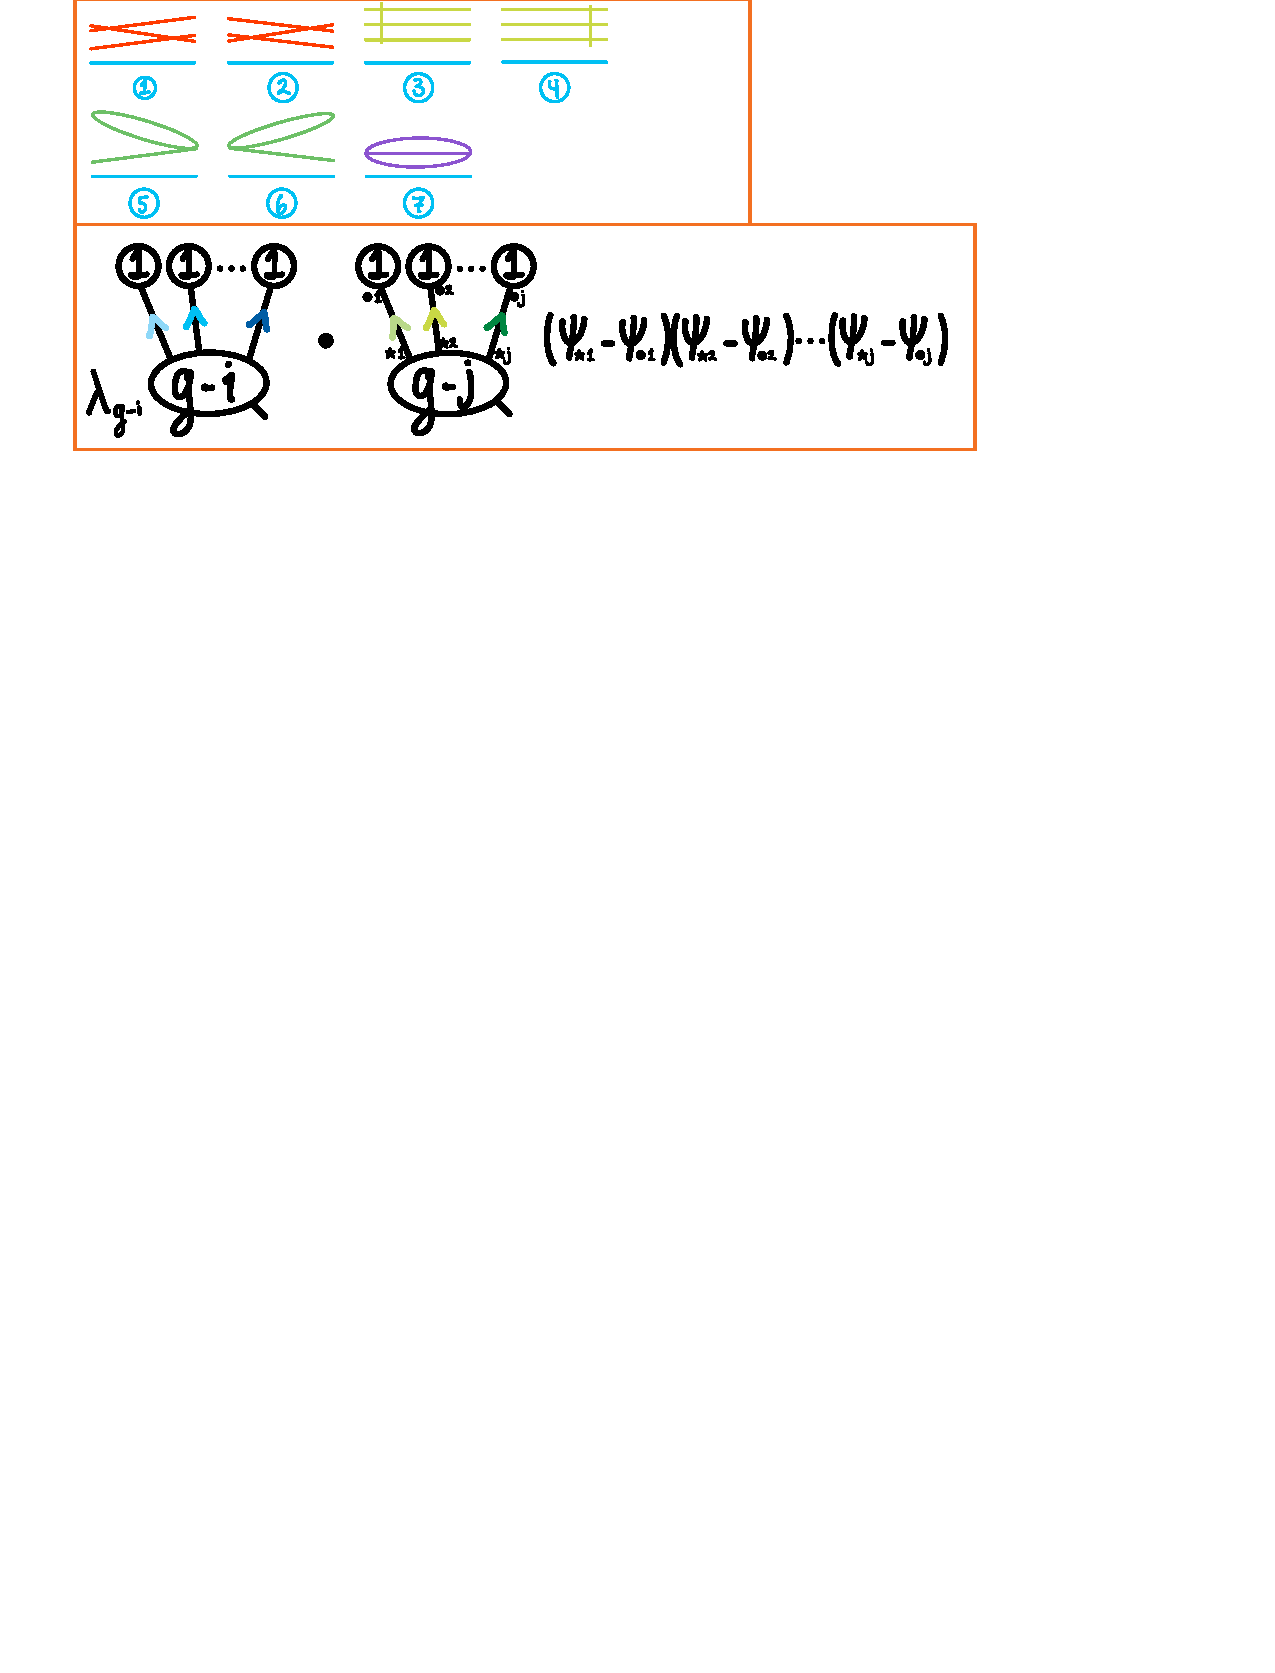
\includegraphics[width=0.8\textwidth, trim= 1.3cm 20.8cm 5.1cm 3.9cm,clip]{figs/FigsDNnotability5.pdf}
        \captionof{figure}{Initial coloring of product}\label{fig:6.2-initial-coloring-glui-times-gluj}
    \end{center}

    Call \(m=\min(i,j)\) and \(M=\max(i,j)\), the product will result in a sum of graphs with the structure of \(\glu_\ast^{M+k}(1)\). In order to color its edges we first color with the one associated with the smaller index, \(m\). There are
    \[
        \binom{M+k}{m}m!\text{ ways to color with }m\text{ colors}.
    \]
    \((M+k)-m\) edges remain unpainted. We have to pick
    \[
        M-((M+k)-m)=m-k
    \]
    edges to paint with the color corresponding to \(M\). Since the colors are distinguishable, we pick
    \[
        \binom{M}{m-k}
    \]
    for the overlap. And there's
    \[
        \binom{m}{m-k}(m-k)!
    \]
    ways to bicolor. Finally the remaining edges can be painted in \((M-m+k)!\) ways. Let \(\text{Bic}\) be the set of bicolored edges, \red{This is wrong as I'm assuming there's more green edges right now}and \(G\) the set of green edges. Our resulting sum of graphs is:
    \[
        \sum_{k=M}^{\min(g,i+j)}a_k\glu^{M+k}_\ast\left(p_0^\ast(\la_{g-(M+k)})\prod_{j\in\text{Bic}}(-\psi_{\star j}^2)\prod_{j\in\text{G}}(\psi_{\star j}p_j^\ast\la_1)\right)
    \]
    where \(a_k\) is the coefficient counting the number of ways to color the graph divided by the automorphisms of the graph.
    \[
        a_k=\frac{\binom{M+k}{m}m!\binom{M}{m-k}\binom{m}{m-k}(m-k)!(M-m+k)!}{(M+k)!}
    \]
    ˝\end{ptcb}

\begin{Ej}
Verify the count via double counting in the other direction. Conclude that the coefficient in question ends up being 
\[
\binom{i}{v}\binom{j}{v}v!,
\]
where \(v\) is the number of vertices in the overlap.
\end{Ej}
\hrule

Taking the integral over \(\ov{M}_{g,1}\) gets us to

\begin{align*}
      & \sum_{k=0}^{g}\frac{d^{2g-2k-2}}{k!}\left(\int_{\ov{M}_{g-k,1+k}}\la_{g-k}\prod_{j=1}^{k}\psi_{\star j}\psi_{P}^{2g-2k-2}\right)\left(\int_{\ov{M}_{1,1}}\la_1\right)^k \\
    = & \sum_{k=0}^{g}\frac{d^{2g-2k-2}}{k!}\frac{(2g-2-k)!}{(2g-2-2k)!}b_{g-k}\frac{1}{24^k}
\end{align*}

Here we applied the \(\la_g\)-conjecture \ref{th-lambdagConj} again to find the value of the first integral. Call this amount \(I_g\). Then our desired \((g_1,g_2)\) contribution is
\[I_{(g_1,g_2)}={d^2}I_{g_1}I_{g_2}.\]

\subsubsection{The \((g,0)\) contribution}

The only difference with the previous calculation lies in the automorphisms bundle. In this case we get an
\[e(\Aut(C))=-t/d\]
which cancels with the \(t/d\) from the curve deformations, and the minus sign cancels out the minus in the \(-t^2\). On the \((0,g)\) case, signs are inverted but the only change is in the psi class in the denominator which doesn't alter the result of the integral. Thus
\[I_{(g,0)}=I_{(0,g)}=I_g\]

\begin{Ej}
    Write this neatly.
\end{Ej}

\subsubsection{The \((g-1,1)\) contribution}

\begin{Ej}
    Prove that
    \[    I_{(g-1,1)}=I_{(1,g-1)}=\frac{d^2-1}{24}I_{g-1}.
    \]
\end{Ej}

\subsubsection{The whole contribution and generating functions}

The full quantity we are looking for is

\begin{align*}
    C^{\ps}(g,d) & =\frac{1}{d}\left(I_{(g,0)}+I_{(g-1,1)}+\dots+I_{(g_1,g_2)}+\dots+I_{(1,g-1)}+I_{(0,g)}\right)                   \\
                 & =\frac{1}{d}\left(I_g+\frac{d^2-1}{24}I_{g-1}+\dots+{d^2}I_{g_1}I_{g_2}+\dots+\frac{d^2-1}{24}I_{g-1}+I_g\right)
\end{align*}

\begin{Qn}
    If such integrals can be extended beyond their just obtained definition, what are \(I_0\) and \(I_1\)? Can we fit them into the sum?
\end{Qn}

\begin{ptcb}
    Observe that

    \begin{align*}
        I_0 & =\sum_{k=0}^{0}\frac{d^{2(0)-2k-2}}{k!}\frac{(2(0)-2-k)!}{(2(0)-2-2k)!}b_{0-k}\frac{1}{24^k} \\
            & =\frac{d^{-2(0)-2}}{0!}\frac{(-2-0)!}{(-2-2(0))!}b_{0}\frac{1}{24^0}                         \\
            & =\frac{b_0}{d^2}=\frac{1}{d^2}
    \end{align*}



    where we have \(b_0=1\) (without using the Bernoulli number definition) and naïvely cancelled the \((-2)!\) on top with the one on the bottom.\par
    On the other hand, for \(I_1\) we compute the two terms of the sum as

    \begin{align*}
        I_1= & \sum_{k=0}^{1}\frac{d^{-2k}}{k!}\frac{(-k)!}{(-2k)!}b_{1-k}\frac{1}{24^k}                                  \\
        =    & \frac{d^{-2(0)}}{0!}\frac{0!}{0!}b_1\frac{1}{24^0} +\frac{d^{-2(1)}}{1!}\frac{(-1)!}{(-2)!}b_0\frac{1}{24} \\
        =    & b_1+\frac{1}{d^2}(-1)\frac{1}{24}                                                                          \\
        =    & \frac{1}{24}-\frac{1}{24d^2}=\frac{d^2-1}{24d^2}
    \end{align*}
    and here we have abused the factorials in the sense that
    \[
        \lim_{n\to-1}\frac{n!}{(n-1)!}=\lim_{n\to-1}n=-1.
    \]

    In this case, \(I_1=\frac{d^2-1}{24d^2}\).

    \iffalse
        so that the sum for \(C^{\ps}(g,d)\) would then fit the pattern a bit more.
        \tcbline
        \emph{Renzo suggests:} Take \(I_0\defeq d^2\) and \(I_1\defeq d^2(d^2-1)/24\) just like that outright. Define them \emph{ad hoc} to fit with the \(1/d^2\) term.
    \fi
\end{ptcb}

Given these two conditions

\[
    \left\lbrace
    \begin{aligned}
         & I_0=1/d^2,          \\
         & I_1=(d^2-1)/(24d^2)
    \end{aligned}
    \right.
    \word{and}
    \left\lbrace
    \begin{aligned}
         & I_{(g,0)}=I_g,                       \\
         & I_{(g-1,1)}=\frac{d^2-1}{24}I_{g-1}, \\
    \end{aligned}
    \right.
\]

these match perfectly when extending the relation \(I_{(g_1,g_2)}=d^2I_{g_1}I_{g_2}\). Observe that

\begin{align*}
     & I_{(g,0)}   =d^2I_gI_0=d^2I_g\left(\frac{1}{d^2}\right)=I_g,                                     \\
     & I_{(g-1,1)} =d^2I_{g-1}I_{1}=d^2I_{g-1}\left(\frac{d^2-1}{24d^2}\right)=\frac{d^2-1}{24}I_{g-1}.
\end{align*}

\begin{Th}
    The generating function for the integrals \(I_g\) is
    \[
        \frac{1}{d^2}\left(1-\frac{t^2}{24}\right)B\left(\frac{dt}{1-{t^2}/{24}}\right),
    \]
    where \(B(t)=\frac{t/2}{\sin\bigl(t/2\bigr)}\) is the generating function for \(b_g\).
\end{Th}

\begin{ptcbp}
    Let us call \(\cI(t)=\sum_{g\geq 0} I_gt^{2g}\), then rewriting \(I_g\) we have
    \[
        \cI(t)=\sum_{g\geq 0} \sum_{k=0}^{g}\frac{d^{2g-2k-2}}{k!}\frac{(2g-2-k)!}{(2g-2-2k)!}b_{g-k}\frac{1}{24^k}t^{2g}.
    \]
    %https://math.stackexchange.com/questions/2558774/using-fubinis-theorem-to-find-an-infinite-sum
    We apply Fubini's theorem to rearrange the sums as
    \[
        \sum_{k\geq 0} \sum_{g=k}^{\infty}\frac{d^{2g-2k-2}}{k!}\frac{(2g-2-k)!}{(2g-2-2k)!}b_{g-k}\frac{1}{24^k}t^{2g}
    \]
    and then take the change of variables \(g=n+k\). From this, as \(g\to k\), \(n\to 0\) and as \(g\) grows, \(n\) also grows. Our sum becomes
    \[
        \sum_{k\geq 0} \sum_{n=0}^{\infty}\frac{d^{2n-2}}{k!}\frac{(2n-2+k)!}{(2n-2)!}b_{n}\frac{1}{24^k}t^{2n+2k}.
    \]
    We may switch order of summation again and manipulate the sum as follows
    \begin{align*}
          & \sum_{n=0}^{\infty}\sum_{k=0}^{\infty}\frac{d^{2n-2}}{k!}\frac{(2n-2+k)!}{(2n-2)!}b_{n}\frac{1}{24^k}t^{2n+2k}  \\
        = & \sum_{n=0}^{\infty}d^{2n-2}b_nt^{2n}\sum_{k=0}^{\infty}\frac{(2n-2+k)!}{(2n-2)!k!}\left(\frac{t^2}{24}\right)^k \\
        = & \sum_{n=0}^{\infty}d^{2n-2}b_nt^{2n}\sum_{k=0}^{\infty}\binom{2n-2+k}{k}\left(\frac{t^2}{24}\right)^k.
    \end{align*}
    The inner sum is very suggestive of the generating function
    \[
        \frac{1}{(1-x)^{m+1}}\sum_{k=0}^{\infty}\binom{m+k}{k} x^k,
    \]
    so that we may rewrite it as
    \begin{align*}
          & \sum_{n=0}^{\infty}d^{2n-2}b_nt^{2n}\frac{1}{\bigl(1-t^2/24\bigr)^{(2n-2)+1}}                         \\
        = & \frac{1}{d^2}\left(1-\frac{t^2}{24}\right)\sum_{n=0}^{\infty}b_n\left(\frac{dt}{1-t^2/24}\right)^{2n} \\
        = & \frac{1}{d^2}\left(1-\frac{t^2}{24}\right)B\left(\frac{dt}{1-t^2/24}\right).
    \end{align*}
    This provees the desired identity.
\end{ptcbp}

\begin{Lem}
    The \(m^{\text{th}}\) derivative of \(1/(1-x)\) is \(\frac{m!}{(1-x)^{m+1}}\) and its generating function is
    \[
        \sum_{k=0}^{\infty}\binom{m+k}{k}m! x^k.
    \]
\end{Lem}

\begin{ptcbp}
    The first part is proved by induction, then
    \begin{align*}
        D^{m}\frac{1}{1-x}        & =\sum_{n=m}^{\infty}n(n-1)\cdots(n-m+1)x^{n-m}            \\
                                  & =\sum_{k=0}^{\infty}(k+m)(k+m-1)\cdots(k+1)x^k            \\
        \To \frac{1}{(1-x)^{m+1}} & =\sum_{k=0}^{\infty}\frac{(k+m)(k+m-1)\cdots(k+1)}{m!}x^k \\
                                  & =\sum_{k=0}^{\infty}\frac{(k+m)!}{k!m!}x^k                \\
                                  & =\sum_{k=0}^{\infty}\binom{m+k}{k} x^k                    \\
    \end{align*}

\end{ptcbp}

We may further simplify the generating function by using the expression for \(B(t)\) as

\[
    \cI(t)=\frac{1}{d^2}\left(1-\frac{t^2}{24}\right)\frac{\frac{dt/2}{1-t^2/24}}{\sin\left(\frac{dt}{2(1-t^2/24)}\right)}=\frac{t/2d}{\sin\left(\frac{dt/2}{1-t^2/24}\right)},
\]

whose first few terms of the expansion are

\begin{align*}
      & \frac{1}{d^{2}} + \frac{(d^{2} - 1) t^{2}}{24 d^{2}} + \frac{(7 d^{2} + 10) t^{4}}{5760} + \frac{(31 d^{4} + 147 d^{2} + 70) t^{6}}{967680} \\
    + & \frac{(381 d^{6} + 3100 d^{4} + 5880 d^{2} + 1400) t^{8}}{464486400}                                                                        \\
    + & \frac{(2555 d^{8} + 29337 d^{6} + 102300 d^{4} + 107800 d^{2} + 15400) t^{10}}{122624409600}+\dots
\end{align*}

% \begin{multline*}
%     \frac{1}{d^{2}} + \frac{(d^{2} - 1) t^{2}}{24 d^{2}} + \frac{(7 d^{2} + 10) t^{4}}{5760} + \frac{(31 d^{4} + 147 d^{2} + 70) t^{6}}{967680} \\
%     + \frac{(381 d^{6} + 3100 d^{4} + 5880 d^{2} + 1400) t^{8}}{464486400} \\
%     + \frac{(2555 d^{8} + 29337 d^{6} + 102300 d^{4} + 107800 d^{2} + 15400) t^{10}}{122624409600} \\
%     + \frac{(1414477 d^{10} + 20925450 d^{8} + 106786680 d^6 + 217217000 d^4 + 147147000 d^2 + 14014000) t^{12}}{2678117105664000} \\
%     + \frac{(860055 d^{12} + 15559247 d^{10} + 104627250 d^8 + 320360040 d^6 + 434434000 d^4 + 206005800 d^2 + 14014000) t^{14}}{64274810535936000} \\
%     + \frac{(355554717 d^{14} + 7602886200 d^{12} + 63481727760 d^{10} + 260870610000 d^8 + 544612068000 d^6 + 531747216000 d^4 + 186778592000 d^2 + 9529520000) t^{16}}{1048964907946475520000} \\
%     + \frac{(5749691557 d^{16} + 141866332083 d^{14} + 1415657410440 d^{12} + 7317327153136 d^{10} + 20817474678000 d^8 + 31870698219360 d^6 + 23574126576000 d^4 + 6387827846400 d^2 + 253485232000) t^{18}}{669659197233029971968000} \\
%     + \frac{(1922471824497 d^{18} + 53759616057950 d^{16} + 624211861165200 d^{14} + 3893057878710000 d^{12} + 14085854769786800 d^{10} + 29768988789540000 d^8 + 35057768041296000 d^6 + 20374780826400000 d^4 + 4391631644400000 d^2 + 139416877600000) t^{20}}{8839501403475995629977600000} \\
%     + \frac{(26880641886945 d^{20} + 840120187305189 d^{18} + 11128240523995650 d^{16} + 81355612571864400 d^{14} + 358161324841320000 d^{12} + 971923979115289200 d^{10} + 1597602398371980000 d^8 + 1497467520621072000 d^6 + 702929938510800000 d^4 + 123453645114800000 d^2 + 3206588184800000) t^{22}}{4879404774718749587747635200000} \\
%     + \frac{(5948296404933711 d^{22} + 205475626583807580 d^{20} + 3058037481790887960 d^{18} + 25654303821317971800 d^{16} + 133260493392713887200 d^{14} + 443260455623617632000 d^{12} + 943414209061240716800 d^{10} + 1246129870730144400000 d^8 + 953886810635622864000 d^6 + 369584941003678400000 d^4 + 53924552186144640000 d^2 + 1167198099267200000) t^{24}}{42626480111942996398563341107200000} \\
%     + O(t^{25})
% \end{multline*}

In order to obtain a generating function for \(C^{\ps}(g,d)\), we recall that

\begin{align*}
    C^{\ps}(g,d) & =\frac{1}{d}\left(I_{(g,0)}+I_{(g-1,1)}+\dots+I_{(g_1,g_2)}+\dots+I_{(1,g-1)}+I_{(0,g)}\right)           \\
                 & =\frac{1}{d}\left(d^2I_gI_0+d^2I_{g-1}I_1+\dots+{d^2}I_{g_1}I_{g_2}+\dots+d^2I_1I_{g-1}+d^2I_0I_g\right) \\
                 & =d\left(I_gI_0+I_{g-1}I_1+\dots+I_{g_1}I_{g_2}+\dots+I_1I_{g-1}+I_0I_g\right)
\end{align*}

so taking the square of \(\cI(t)\) and multiplying by \(d\) gets us

\begin{align*}
    d\cI(t)^2     & =d\sum_{g\geq 0} \left(\sum_{\substack{g_1+g_2=g                                                                             \\ g_1,g_2\geq 0}}I_{g_1}I_{g_2}\right)t^{2g}\\
                  & =\sum_{g\geq 0} d\left(\sum_{\substack{g_1+g_2=g                                                                             \\ g_1,g_2\geq 0}}I_{g_1}I_{g_2}\right)t^{2g}\\
    \To d\cI(t)^2 & =\sum_{g\geq 0} C^{\ps}(g,d)t^{2g}                                                                                           \\
    \To\cC(t)     & =d\left(\frac{t/2d}{\sin\left(\frac{dt/2}{1-t^2/24}\right)}\right)^2=\frac{t^2/4d}{\sin^2\left(\frac{dt/2}{1-t^2/24}\right)} \\
\end{align*}

The first few terms of this sum are

\begin{align*}
      & \frac{1}{d^{3}} + \frac{(d^{2} - 1) t^{2}}{12 d^{3}} + \left(\frac{1}{576 d^{3}} + \frac{d}{240}\right) t^{4} + \frac{d (10 d^{2} + 21) t^{6}}{60480} \\
    + & \frac{d (84 d^{4} + 400 d^{2} + 315) t^{8}}{14515200} + \frac{d (180 d^{6} + 1386 d^{4} + 2750 d^{2} + 1155) t^{10}}{958003200}+\dots
\end{align*}

% \begin{multline*}
%     \frac{1}{d^{3}} + \frac{(d^{2} - 1) t^{2}}{12 d^{3}} + \left(\frac{1}{576 d^{3}} + \frac{d}{240}\right) t^{4} + \frac{d (10 d^{2} + 21) t^{6}}{60480} \\
%     + \frac{d (84 d^{4} + 400 d^{2} + 315) t^{8}}{14515200} + \frac{d (180 d^{6} + 1386 d^{4} + 2750 d^{2} + 1155) t^{10}}{958003200} \\
%     + \frac{d (243232 d^{8} + 2620800 d^{6} + 8828820 d^{4} + 10010000 d^{2} + 2627625) t^{12}}{41845579776000} \\
%     + \frac{d (17472 d^{10} + 243232 d^{8} + 1179360 d^{6} + 2354352 d^{4} + 1751750 d^{2} + 315315) t^{14}}{100429391462400} \\
%     + \frac{d (2083392 d^{12} + 35642880 d^{10} + 227421920 d^{8} + 668304000 d^{6} + 900539640 d^{4} + 476476000 d^{2} + 62537475) t^{16}}{409751917166592000} \\
%     + \frac{d (23863648 d^{14} + 484909488 d^{12} + 3851658720 d^{10} + 15123557680 d^{8} + 30554023500 d^{6} + 29942943030 d^{4} + 11882120250 d^{2} + 1188212025) t^{18}}{163491014949470208000} \\
%     + \frac{d (35670931968 d^{16} + 840000409600 d^{14} + 8001006552000 d^{12} + 39543696192000 d^{10} + 108133437412000 d^{8} + 161325244080000 d^{6} + 120769870221000 d^{4} + 37343806500000 d^{2} + 2940824761875) t^{20}}{8632325589332026982400000} \\
%     + \frac{d (275631713280 d^{18} + 7383882917376 d^{16} + 82110040038400 d^{14} + 490728401856000 d^{12} + 1705321898280000 d^{10} + 3481896684666400 d^{8} + 4019687331660000 d^{6} + 2380891727214000 d^{4} + 590498940281250 d^{2} + 37577205290625) t^{22}}{2382521862655639447142400000} \\
%     + \frac{d (33401082427392 d^{20} + 1003299436339200 d^{18} + 12766733564143104 d^{16} + 89664163721932800 d^{14} + 379578418835616000 d^{12} + 993179473558272000 d^{10} + 1584262991523212000 d^{8} + 1463166188724240000 d^{6} + 704148728323540500 d^{4} + 143294409508250000 d^{2} + 7522956499183125) t^{24}}{10406855496079833105118003200000} \\
%     + O(t^{25})
% \end{multline*}

\subsection{Differential equations and Virasoro constraints}

The function \(B(t)=\frac{t/2}{\sin(t/2)}\) satisfies the differential equation 

\[
y''+\cot\left(\frac{t}{4}\right)y'-\frac{y}{4}=0,\quad y(0)=1,\quad y'(0)=0.
\]

If we call \(T=\frac{t}{1-t^2/24}\), then \(\cI(t)=\frac{t}{d^2T}B(dT)\) and \(\cC(t)=\frac{t^2}{d^3T^2}B(dT)^2\).

\begin{Qn}
    Based on this information,
    \begin{enumerate}
        \item can we find a differential equation satisfied by \(\cI(t)\), and
        \item can we show that \(\cI(t)\) or \(\cC(t)\) satisfy a modified version of the Virasoro constraints?
    \end{enumerate}
    More importantly, we must understand first what the Virasoro constraints are.
\end{Qn}

\end{document}